\documentclass{article}

\usepackage{arxiv}

\usepackage[utf8]{inputenc} % allow utf-8 input
\usepackage[T1]{fontenc}    % use 8-bit T1 fonts
\usepackage{hyperref}       % hyperlinks
\usepackage{url}            % simple URL typesetting
\usepackage{booktabs}       % professional-quality tables
\usepackage{amsfonts}       % blackboard math symbols
\usepackage{nicefrac}       % compact symbols for 1/2, etc.
\usepackage{microtype}      % microtypography
\usepackage{lipsum}
\usepackage{graphicx}
\usepackage{gensymb}
\usepackage{float}

\usepackage{listings}
\usepackage{xcolor}

\definecolor{codegreen}{rgb}{0,0.6,0}
\definecolor{codegray}{rgb}{0.5,0.5,0.5}
\definecolor{codepurple}{rgb}{0.58,0,0.82}
\definecolor{backcolour}{rgb}{0.95,0.95,0.92}

\lstdefinestyle{mystyle}{
    backgroundcolor=\color{backcolour},   
    commentstyle=\color{codegreen},
    keywordstyle=\color{magenta},
    numberstyle=\tiny\color{codegray},
    stringstyle=\color{codepurple},
    basicstyle=\ttfamily\footnotesize,
    breakatwhitespace=false,         
    breaklines=true,                 
    captionpos=b,                    
    keepspaces=true,                 
    numbers=left,                    
    numbersep=5pt,                  
    showspaces=false,                
    showstringspaces=false,
    showtabs=false,                  
    tabsize=2
}

\lstset{style=mystyle}

\graphicspath{ {./images/} }

\title{Contare monete con un Arduino Nano}

\author{
 Matteo Galiazzo \\
  Dipartimento di Informatica - Scienza e Ingegneria\\
  Università di Bologna\\
  \texttt{matteo.galiazzo@studio.unibo.it} \\
  %% examples of more authors
%    \And
%  Zixuan Lu \\
%   School of Coumputing and Information\\
%   University of Pittsburgh\\
%   Pittsburgh, PA 15213 \\
%   \texttt{ZIL50@pitt.edu} \\
%   \And
%  Yuchen Lu \\
%   School of Coumputing and Information\\
%   University of Pittsburgh\\
%   Pittsburgh, PA 15213 \\
%   \texttt{yul217@pitt.edu} \\
  %% \AND
  %% Coauthor \\
  %% Affiliation \\
  %% Address \\
  %% \texttt{email} \\
  %% \And
  %% Coauthor \\
  %% Affiliation \\
  %% Address \\
  %% \texttt{email} \\
  %% \And
  %% Coauthor \\
  %% Affiliation \\
  %% Address \\
  %% \texttt{email} \\
}

\begin{document}
\maketitle
\begin{abstract}
In questo progetto è stato realizzato un contamonete a basso costo, con l'obiettivo di sviluppare un dispositivo funzionale simile a quelli professionali reperibili in commercio, ma a un prezzo notevolmente inferiore.  
La struttura principale è stata progettata con Fusion360 e realizzata in legno. Per la raccolta delle monete sono stati stampati in 3D cassettini dedicati.  
Il riconoscimento delle monete è stato implementato mediante sensori a infrarossi collegati a un microcontrollore Arduino Nano.  
\end{abstract}


\tableofcontents

\section{Introduzione}
Cercando online, come si può vedere in \ref{fig:contamonete_professionale}, un contamonete professionale si trova a partire da circa 100 euro.
Lo scopo del progetto è di realizzare un dispositivo equivalente a un costo minore.

\begin{figure}[h] % htbp
  \centering
  \includegraphics[width=0.8\linewidth]{./images/contamonete_professionale.png}
  \caption{}
  \label{fig:contamonete_professionale}
\end{figure}

\section{Materiali utilizzati}
Per la realizzazione del progetto sono stati usati:
\begin{itemize}
    \item Componenti elettronici
    \begin{itemize}
        \item 1 Arduino Nano
        \item 5 sensori a infrarossi
        \item 1 breadboard
        \item cavetti colorati
    \end{itemize}
    \item Macchinari e utensili per la lavorazizone del legno
    \begin{itemize}
        \item CNC MasterWood Project 313
        \item Sega circolare da banco
        \item Carta vetrata
        \item Adesivo vinilico UniCol
    \end{itemize}
    \item Materiali
    \item \begin{itemize}
        \item Pannello 2x3 metri compensato spessore 6 mm
        \item 4 Pannelli 40x40 cm MDF
    \end{itemize}
    \item Stampante 3D Elegoo Centauri Carbon
    \item Filamento PLA rosso
\end{itemize}

\section{Software utilizzati}
Per la realizzazione del progetto è stato utilizzato:
\begin{itemize}
    \item Fusion360
    \item Arduino IDE
\end{itemize}

\section{Progettaizone e realizzazione slider in legno}
Come prima cosa sono partito dalla progettazione dello slider, cioè la parte in legno dove le monete scivolano per cadere nei vari buchi.
Mi sono ispirato a un modellino in cartone che avevo realizzato qualche anno fa, che si può vedere in figura \ref{fig:prototipo}.

\begin{figure}[htbp]
  \centering
  \includegraphics[width=0.8\linewidth]{./images/prototipo.png}
  \caption{}
  \label{fig:prototipo}
\end{figure}

Con Fusion360 ho modellato lo slider, aggiungendo degli accorgimenti rispetto al prototipo in cartone, come si vede in figura \ref{fig:screen_slider}.

\begin{figure}[htbp]
  \centering
  \includegraphics[width=0.8\linewidth]{./images/screen_slider.png}
  \caption{}
  \label{fig:screen_slider}
\end{figure}

Dal modello 3D, dato che ho dovuto tagliare i pezzi di legno per comporre la struttura, ho ricavato una tavola da disegno utilizzando gli strumenti predefiniti di Fusion360, che si può vedere in figura \ref{fig:tavola_slider}.

\begin{figure}[htbp]
  \centering
  \includegraphics[width=0.8\linewidth]{./images/tavola_slider.png}
  \caption{}
  \label{fig:tavola_slider}
\end{figure}

Avendo il disegno completo, e quindi sapendo chiaramente come andavano tagliati e assemblati i pezzi sono andato in falegnameria a tagliarli.
In falegnameria avevo a disposizione una macchina a controllo numerico computerizzato (CNC).
La macchina, essendo del 1995 andava programmata tramite un terminale che accettava istruzioni G-code, un linguaggio utilizzato per le macchine a controllo numerico.
Per il taglio di pezzi semplici come quello che dovevo realizzare io, bastava dare una posizione di partenza con il comando \verb|G72|, e poi muoversi con il comando \verb|G01|.
Per esempio:
\begin{lstlisting}
G72 X26 Y26 Z3 S18 E1 T41
G01 X26 Y120 Z3 Q5 F1
\end{lstlisting}
Il seguente comando posiziona la fresa a 26 mm dagli assi x e y, e poi fa un movimento in linea retta (dato che la coordinata x rimane invariata) di 94 mm verso il basso con velocità (Speed) 18 e lo strumento (Tool) 41. La lettera \verb|E| indica che il comando va eseguito 1 volta sola.
\verb|Q5| serve invece a dare l'angolo di quadratura (quanto smussare l'angolo), e \verb|F1| controlla il Feedrate, cioè la velocità della fresa.
Va notato che il comando prende il centro della fresa come riferimento, e quindi sta a chi programma la macchina stare attento a tenere conto del diametro della fresa nella programmazione della macchina.
Per esempio quindi, per fare un taglio di 100 mm di lunghezza con una fresa di 8 mm di diametro partendo a 40 mm dall'asse bisogna poi spostarsi di $100 - 8$ mm.
Possiamo vedere questo programma in figura \ref{fig:programma_cnc}

\begin{figure}[htbp]
  \centering
  \includegraphics[width=0.8\linewidth]{./images/programma_cnc.png}
  \caption{}
  \label{fig:programma_cnc}
\end{figure}

Dato che i pezzi sono molto piccoli, per non danneggiare le piastre con le ventose sulla macchina, ho incollato con del nastro biadesivo i pannelli di compensato a dei pannelli spessi di MDF, che poi venivano posizionati sulla macchina, come si vede in figura \ref{fig:mdf_compensato}.

\begin{figure}[htbp]
  \centering
  \includegraphics[width=0.8\linewidth]{./images/mdf_compensato.png}
  \caption{}
  \label{fig:mdf_compensato}
\end{figure}

Come ultima cosa prima di incollare i pezzi, ho tagliato i laterali a $22 \degree$, di modo che si potesse appoggiare il piano per lo scivolamento.
Dopodichè ho incollato i vari pezzi come da progettazione, utilizzando la colla vinilica.

\begin{figure}[htbp]
  \centering
  \includegraphics[width=0.8\linewidth]{./images/slider_finito.png}
  \caption{}
  \label{fig:slider_finito}
\end{figure}

In figura \ref{fig:slider_finito} si può vedere lo slider in legno finito, di fianco al suo prototipo.

Per raccogliere le monete ho realizzato tramite stampa 3D 5 cassettini identici, di dimensione $45 \times 80 \times 43$.
I cassettini sono stati modellati con Fusion360 ed esportati in \verb|stl|. Poi tramite Prusa Slicer ho piazzato i cassettini sul piatto di stampa e selezionato l'infill 10\%.
La prima stampa è fallita dato che stampando contemporaneamente i 5 cassettini il filamento del 1$\degree$ cassettino diventava troppo freddo nel tempo in cui la stampante creava gli altri 4, e quindi i cassettini si sono deformati.
Avrei quindi dovuto utilizzare una temperatura del piatto più alta rispetto ai 35$\degree$ di default, di modo da mantenere il filamento in temperatura.

Si possono vedere i cassettini finiti in figura \ref{fig:cassettino}

\begin{figure}[htbp]
  \centering
  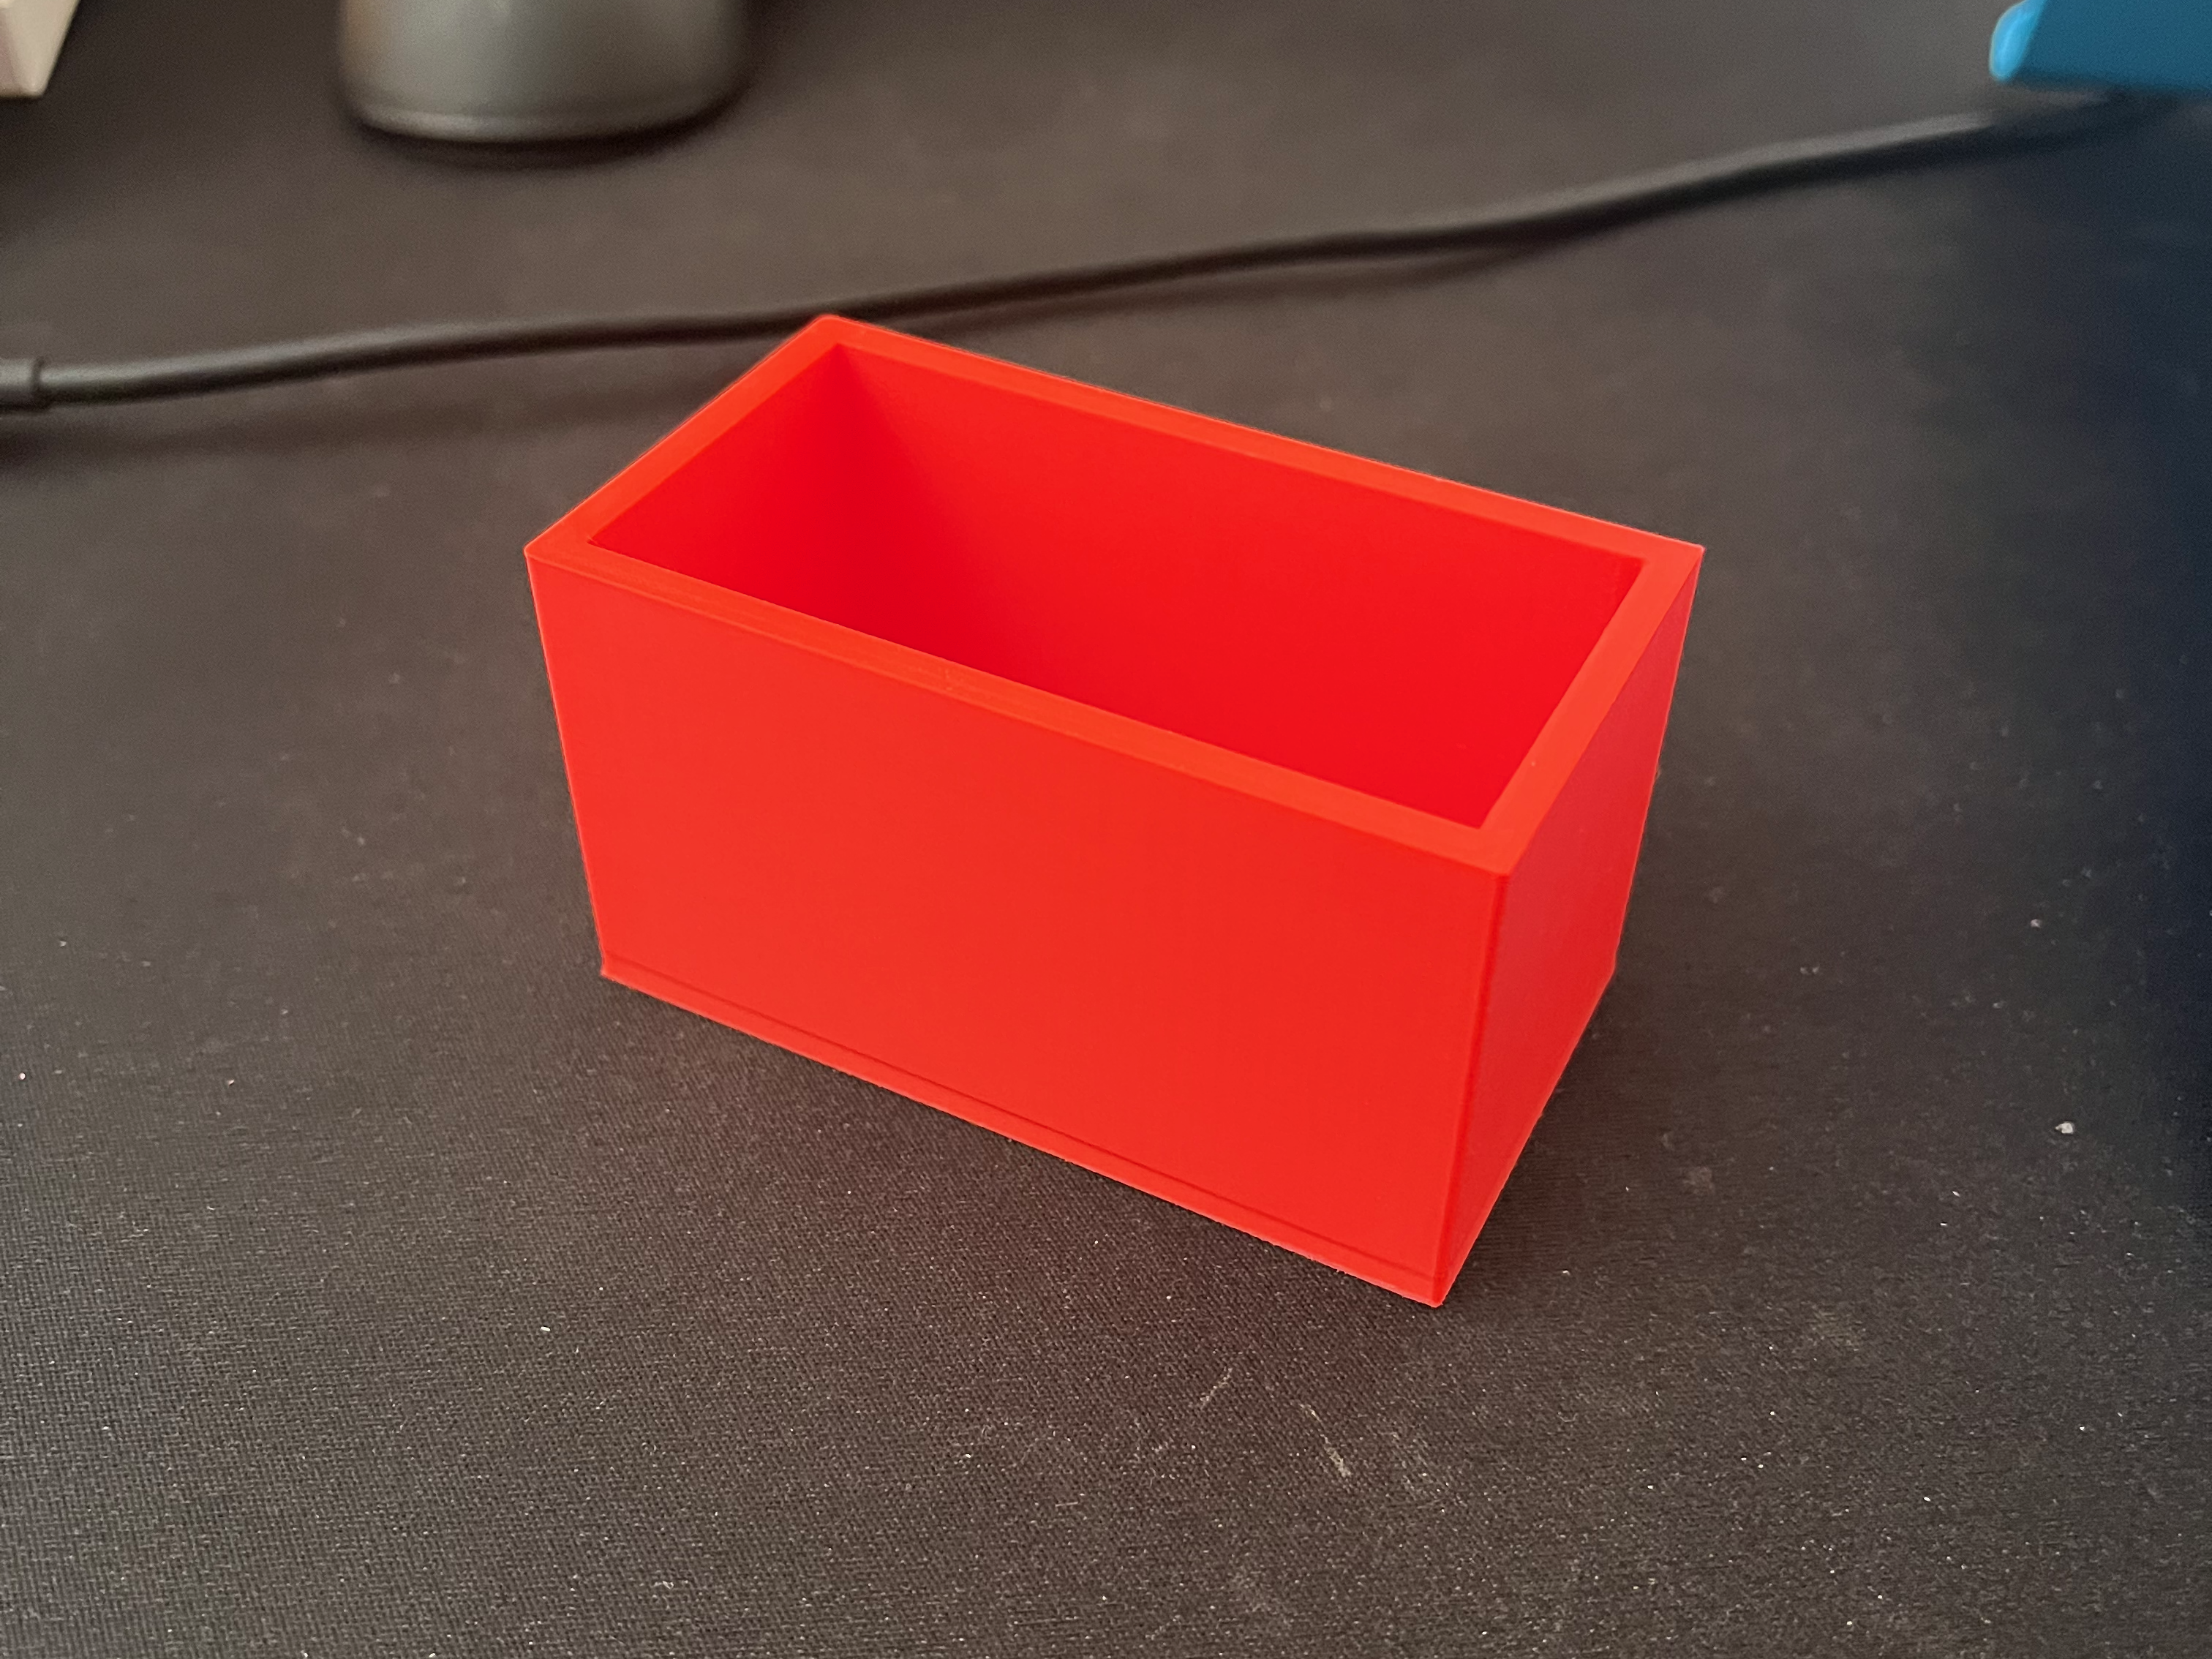
\includegraphics[width=0.8\linewidth]{./images/cassettino.png}
  \caption{}
  \label{fig:cassettino}
\end{figure}

\section{Progettazione e realizzazione circuito e software}

La progettazione del circuito elettrico è iniziata con un prototipo, per testare i sensori a infrarossi.
Dalla pagina del prodotto su AliExpress si può leggere che i sensori possono essere alimentati sia a 5 V che a 3.3 V, e dato che ho visto che a 3.3 V i sensori erano meno sensibili (penso perchè essendo alimentati con meno tensione il sensore emetteva meno raggi a infrarossi, che quindi venivano più difficilmente riflessi, e quindi rilevati) li ho utilizzati direttamente a 5V, senza resistenze di carico nel mezzo.
Si può vedere il circuito finito in figura \ref{fig:circuito_finito}.

\begin{figure}[htbp]
  \centering
  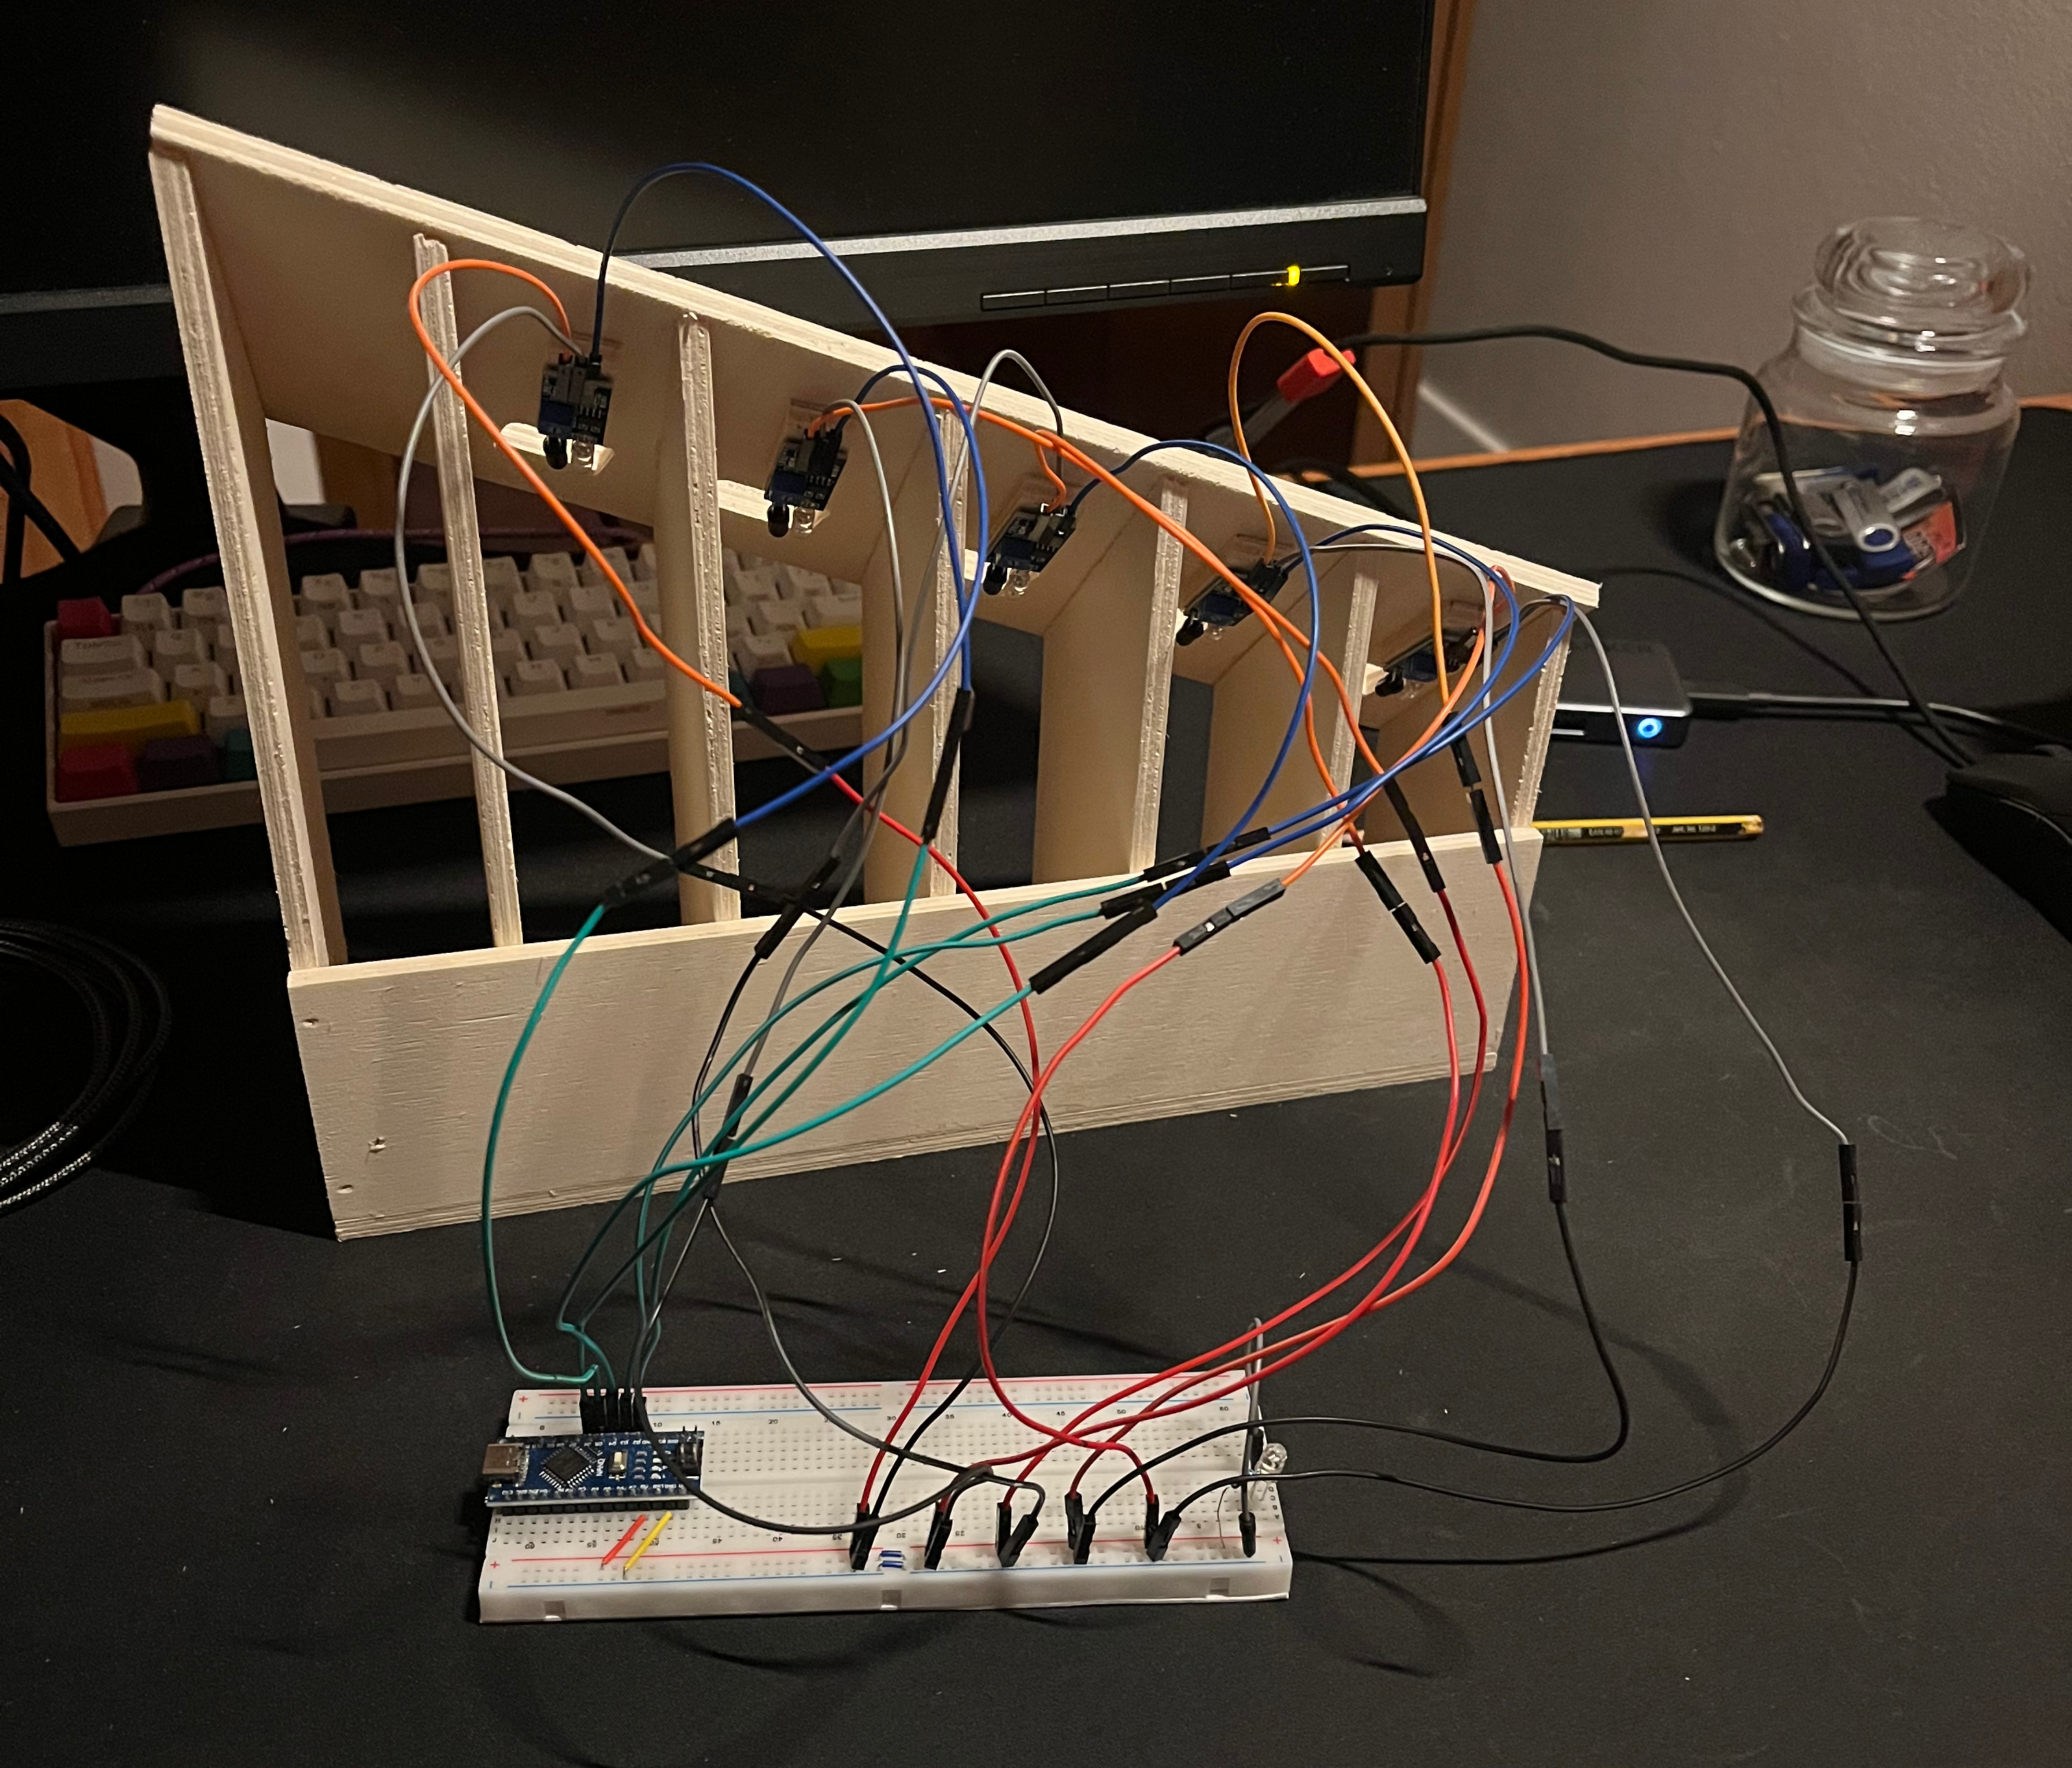
\includegraphics[width=0.8\linewidth]{./images/circuito_finito.png}
  \caption{}
  \label{fig:circuito_finito}
\end{figure}

I sensori sono stati collegati sui pin dal \verb|D2| al \verb|D6| nell'Arduino.
Il software è molto semplice.
Nel \verb|loop|, a ogni iterazione viene letto il tempo corrente e i valori associati a ogni sensore.
Dopodichè, una funzione per ogni tipo di moneta rilevabile controlla se la moneta è stata rilevata e se non è in cooldown.

\begin{lstlisting}[language=C++]
// --- Process 2 Euro Coin Sensor ---
if (prev_2euro_state == HIGH && current_2euro_state == LOW) {
    if (current_time - last_2euro_time > COOLDOWN_MS) {
        counter_2euro++;
        last_2euro_time = current_time;
        Serial.print("2 Euro coin detected!   |  Total: ");
        Serial.println(getTotal(), 2);
    }
}
prev_2euro_state = current_2euro_state;
\end{lstlisting}
Questo è necessario perchè durante la caduta una moneta potrebbe, mentre sta ruotando, attivare 2 volte il sensore, e quindi venire conteggiata 2 volte.
Aggiungendo un cooldown di 150 ms evitiamo che una moneta venga conteggiata 2 volte, ma riuscendo comunque a contare 2 monete dello stesso tipo che cadono in modo consecutivo.

\vspace{1em}

Possiamo vedere lo slider con i cassettini completato in figura \ref{fig:slider_cassetti_finito}
\begin{figure}[htbp]
  \centering
  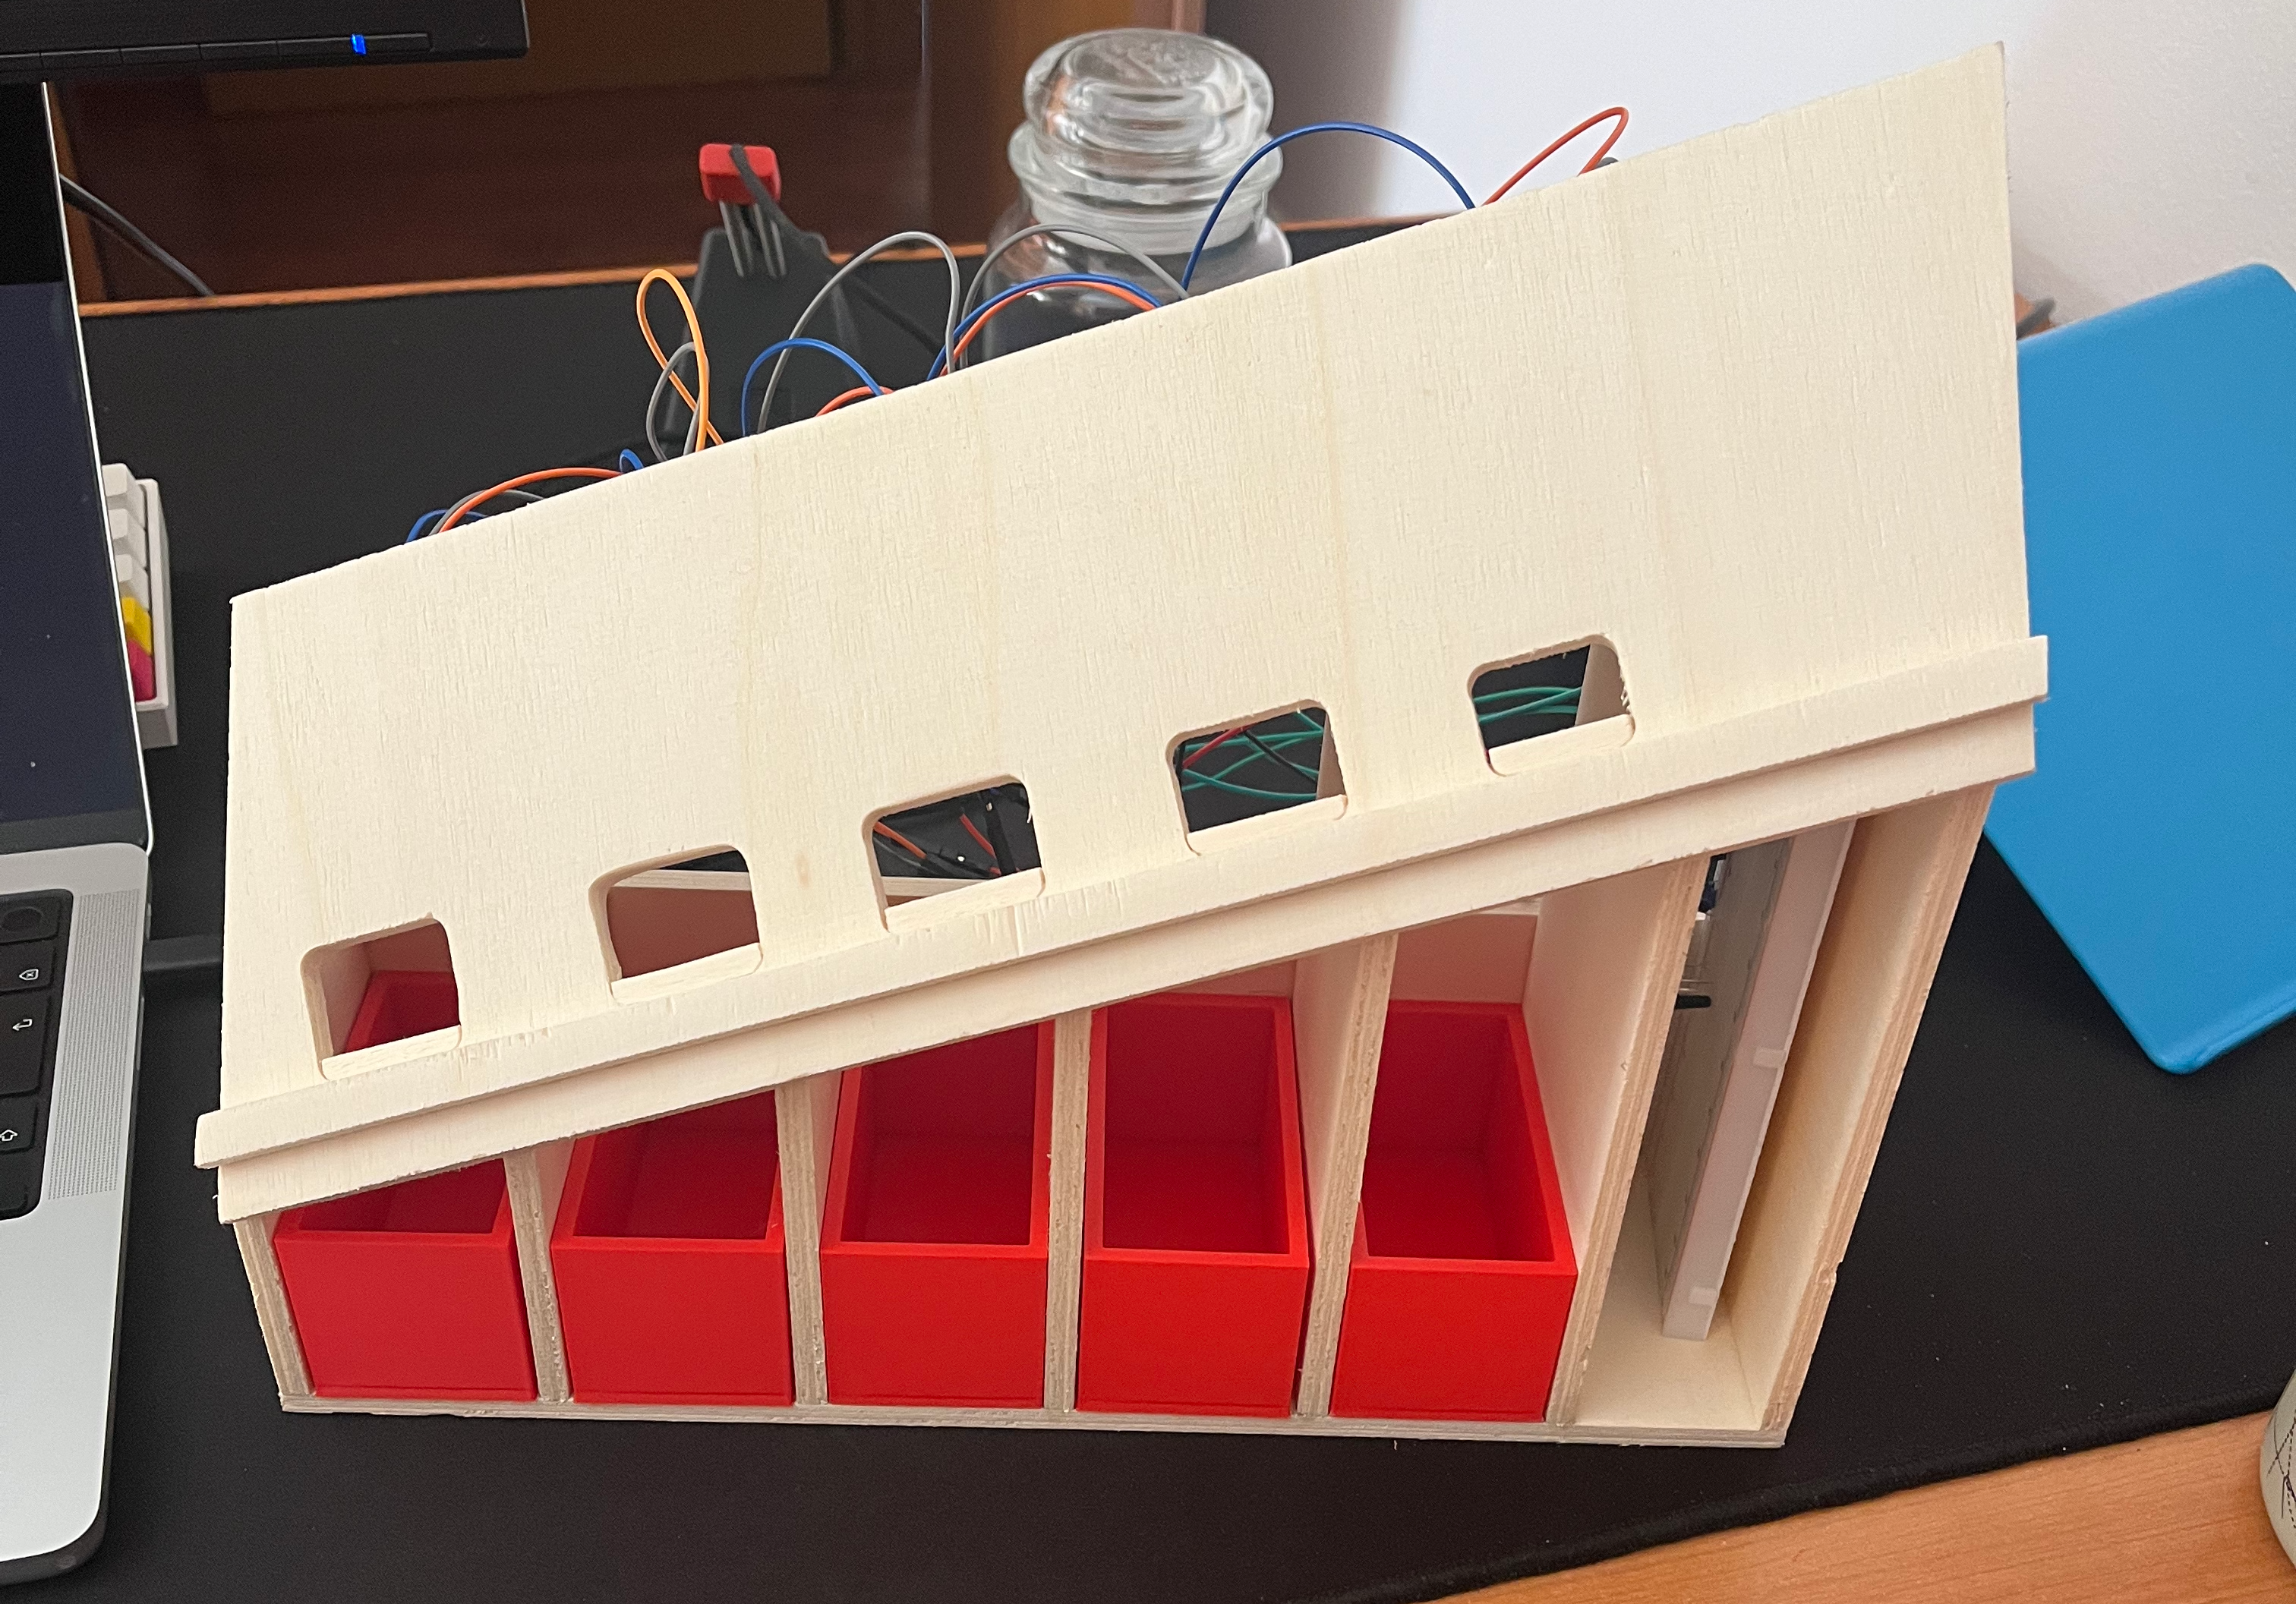
\includegraphics[width=0.8\linewidth]{./images/slider_cassetti_finito.png}
  \caption{}
  \label{fig:slider_cassetti_finito}
\end{figure}

\end{document}
